% This file contains the frontpage of the report.

% Titel, illustration, forfattere, fag, skolens navn og årstal skal fremgå 

\title{\doctitle}
\author{\docauthor}
\date{\docdate}

\newgeometry{left=10mm,right=10mm,top=20mm,bottom=0pt,bindingoffset=0mm,footskip=0mm}

\begin{titlepage}
	\pagecolor{\maincolour}
	\thispagestyle{empty}

	\begin{tikzpicture}[remember picture,overlay]

		% HCØ logo
		\node[anchor=north west,
			yshift=6mm]
		at (current page text area.north west)
		{\includesvg[height=14mm,keepaspectratio]{graphics/HCO.svg}};

		% Institution
		\node[anchor=north east,
			yshift=6mm,
			color=white]
		at (current page text area.north east)
		{
			\begin{tabular}{r}
				{\NeoSansProMed \docauthorgym} \\
				{\NeoSansProReg \docproject}
			\end{tabular}
		};

		% Title
		\node[anchor=north west,
			xshift=0mm,
			yshift=-30mm,
			text width=\textwidth,
			color=white]
		at (current page text area.north west)
		{
			\Huge
			\begin{tabular}{p{\linewidth}}
				{\NeoSansProMed \doctitle} \smallskip \\
				{\NeoSansProReg \docsubtitle}
			\end{tabular}
		};

		% Cover photo
		\node[anchor=south,
			xshift=0pt,
			yshift=-2.9mm] % shifting picture to actually be at the bottom of the page
		(bg) at (current page.south)
		{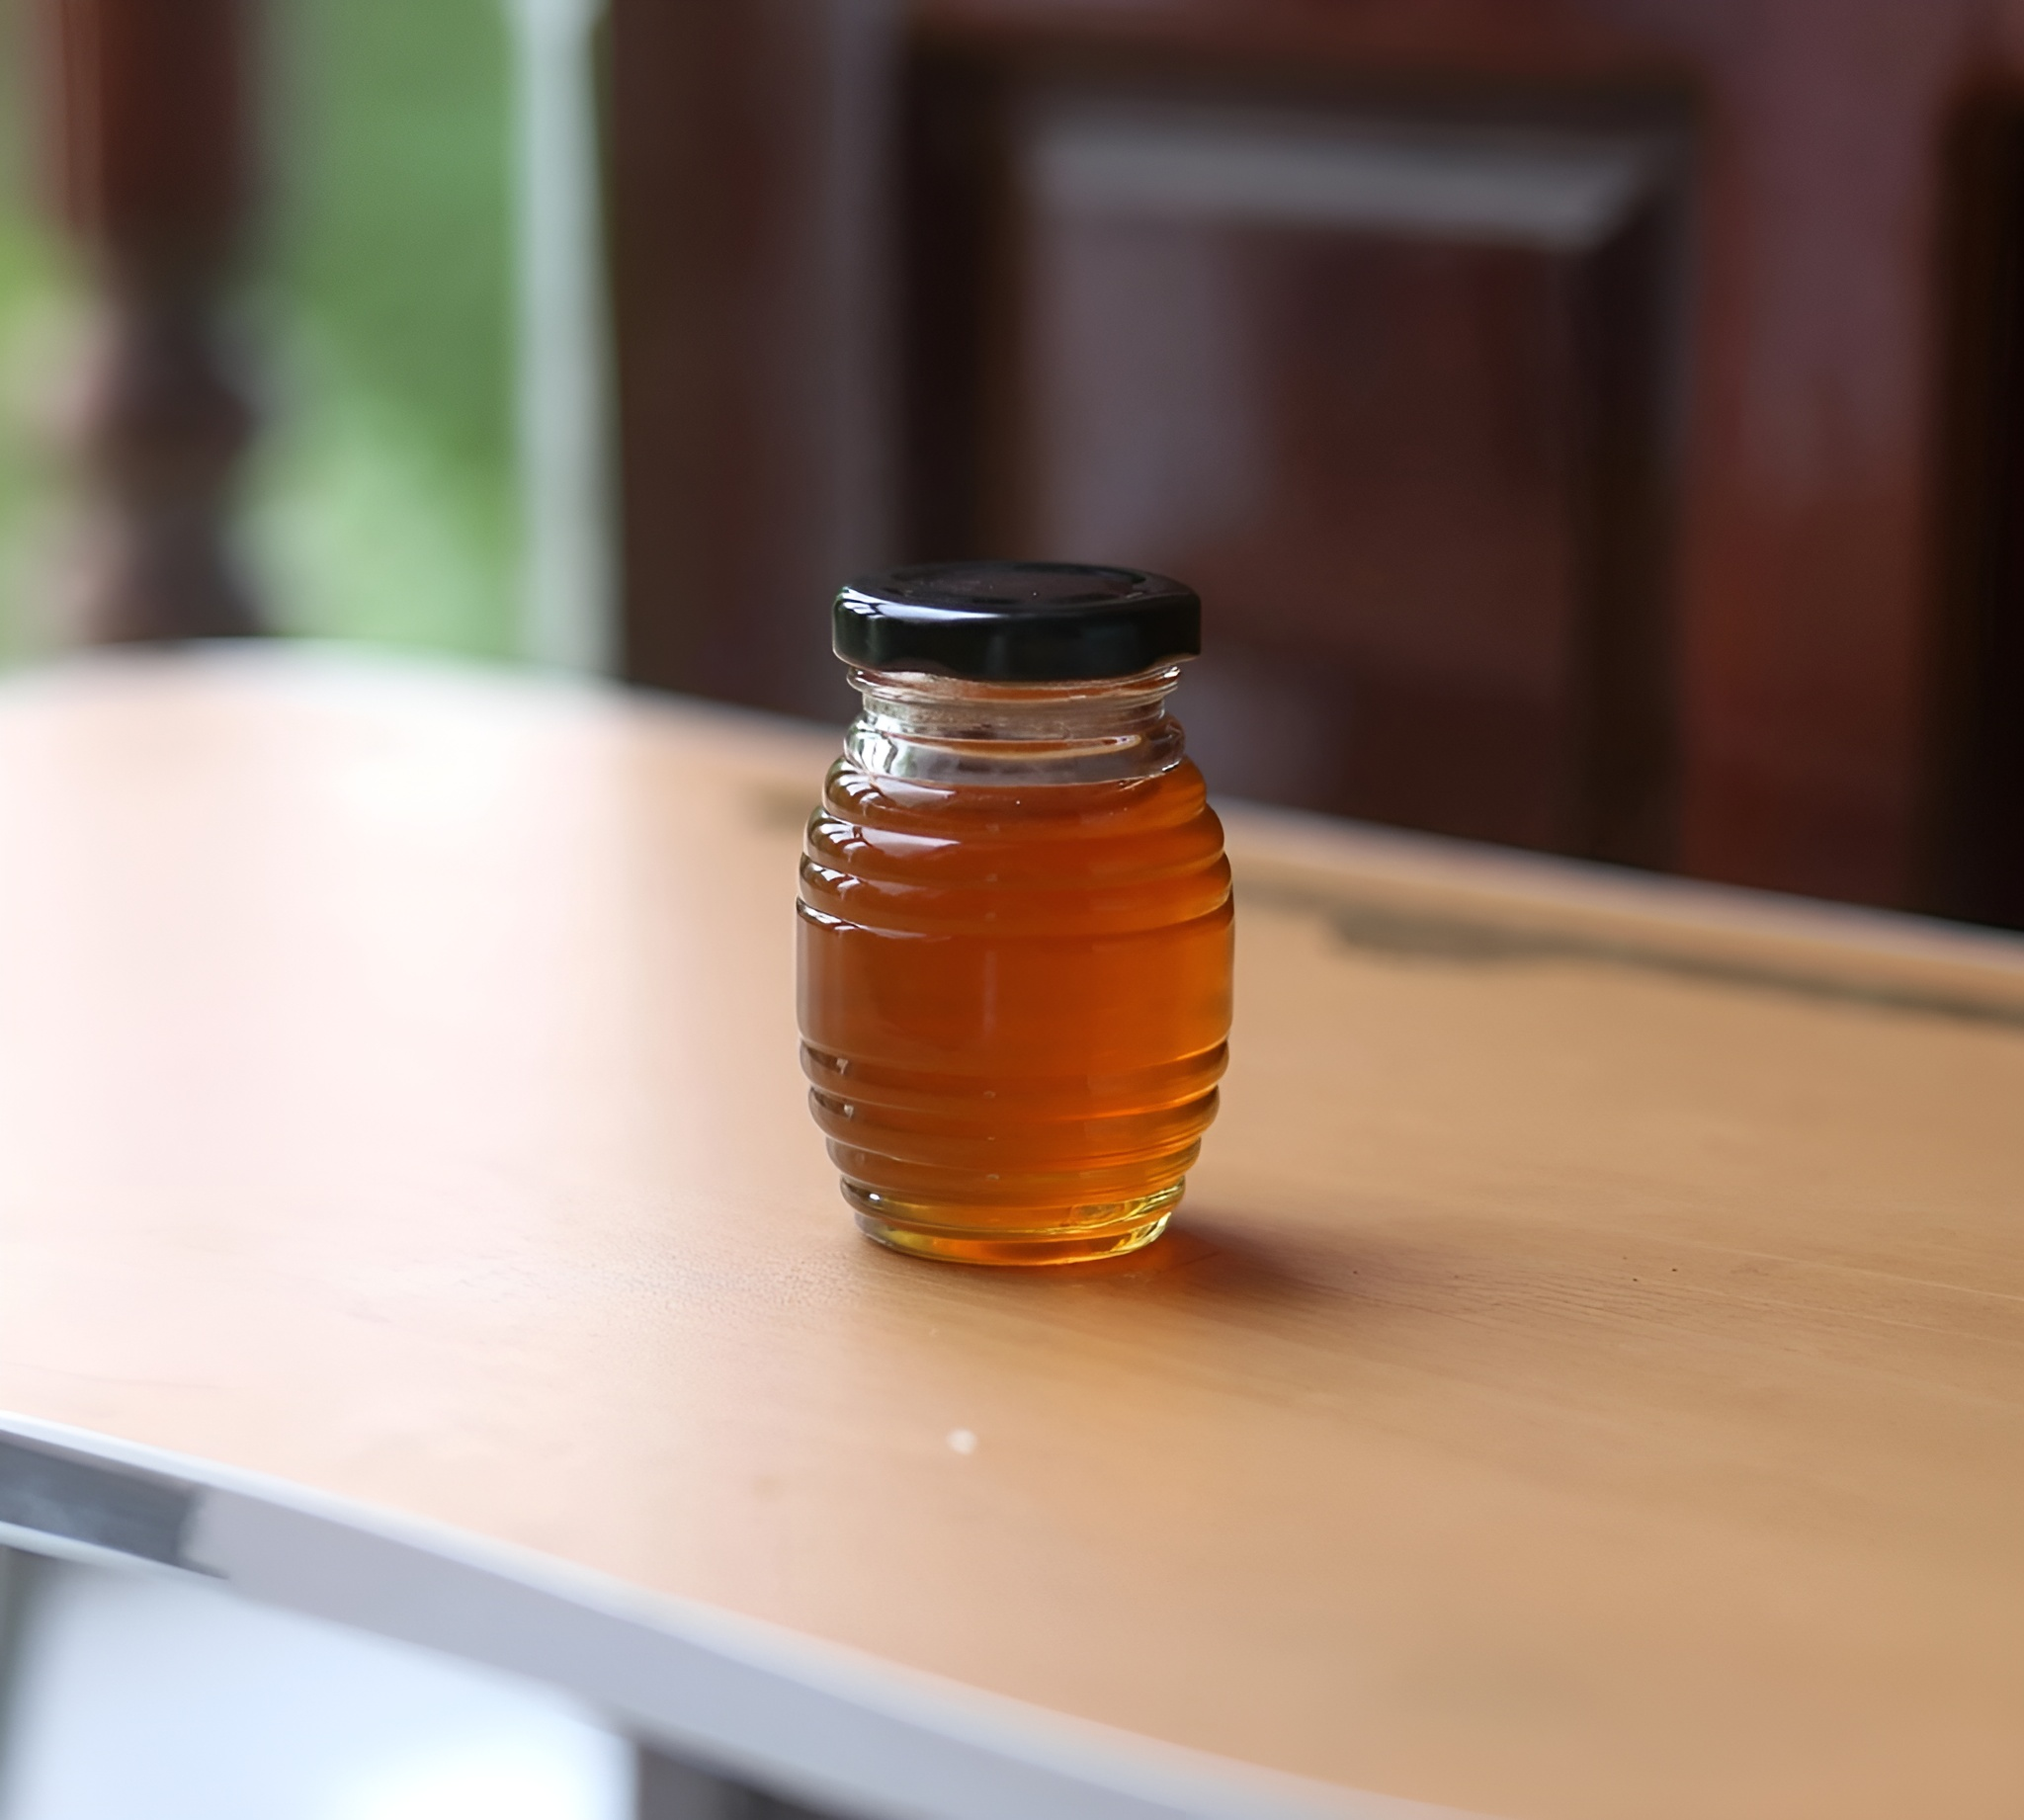
\includegraphics[height=18.9cm,keepaspectratio]{honey-jar.png}};

		% Author 
		\node[anchor=south west,
			xshift=10mm,
			yshift=3mm,
			color=white]
		at (bg.north west)
		{
			\begin{tabular}{l}
				{\NeoSansProMed \docauthor}
			\end{tabular}
		};

		% Year
		\node[anchor=south east,
			xshift=-10mm,
			yshift=3mm,
			color=white]
		at (bg.north east)
		{
			\begin{tabular}{r}
				{\NeoSansProReg \docdate}
			\end{tabular}
		};

	\end{tikzpicture}
\end{titlepage}

